% -----------------------------------------------------------------------------
\section{SBOL Glyphs}\label{sec:glyphs}
% -----------------------------------------------------------------------------

A glyph is a visual symbol used to represent an element in an SBOL Visual diagram.
All of the currently defined glyphs are collected in \ref{apdx:symbols}.
%
This section explains how glyphs are specified and how to add new glyphs.

Each SBOL glyph is defined by association with ontology terms, and can be used to represent any nucleic acid sequence feature that is well-described by that term.  
For SBOL 2 data models, this is formally defined as any \sbol{Component} with a compatible term within its \sbol{roles},
 i.e. one that is equal to or a child of at least one term associated with the glyph.
 
More than one glyph may share the same definition: in this case, these glyphs form a family of variants, of which precisely one MUST be designated as the RECOMMENDED glyph, which is to be used unless there are strong reasons to prefer an alternative variant.

It will also frequently be the case that a sequence feature could be represented by more than one glyph (e.g., a glyph for a specific term and a glyph for a more general term).
In such cases, it is RECOMMENDED that the most specific applicable glyph be used.

For example, a CDS may be represented as either using the CDS glyph (Sequence Ontology term SO:0000316) or the Unspecified glyph (Sequence Ontology term SO:0000001).  
Since SO:0000316 is contained by SO:0000001, the preferred glyph is CDS, rather than Unspecified.
Likewise, a CDS may be represented by either a pentagonal glyph or an arrow glyph, but the pentagon is the RECOMMENDED variant, and so it is likewise preferred.  
\ref{f:glyphalternatives} illustrates this example.

\begin{figure}[h!]
\centering
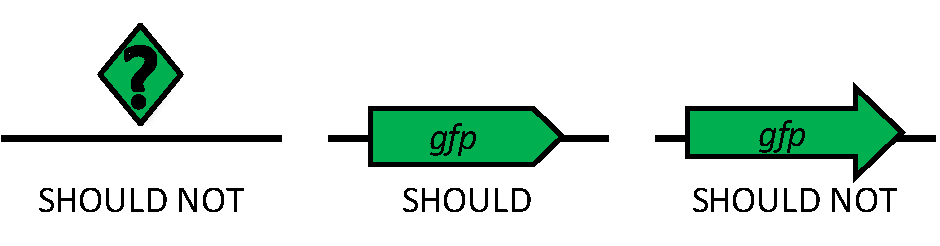
\includegraphics[scale=0.6]{figures/glyphalternatives.pdf}
\caption{A biological design element such as a protein coding sequence (CDS) is best represented by the most specific RECOMMENDED glyph (middle), but can be represented by a less specific glyph such as Unspecified (left) or an approved alternative glyph (right).}
\label{f:glyphalternatives}
\end{figure}

\subsection{Requirements for Glyphs}

A number of requirements are placed on SBOL Visual glyphs in order to
ensure both the clarity of diagrams and the ease with which they can
be constructed:
\begin{enumerate}
\item A glyph SHOULD have its meaning defined by associating the glyph with at least one ontology definition.
	Definitions are RECOMMENDED to be from the Sequence Ontology for nucleic acid components and from Systems Biology Ontology for other components and interactions.  
	If no applicable terms are available in the preferred ontology, proposal of a new glyph SHOULD be accompanied by a request to the ontology maintainers to add a term for the undefined entity.  
\item A glyph MUST be relatively easy to sketch by hand (e.g., no high-complexity images or precise angles required).
\item A glyph specification MUST include a rectangular bounding box indicating its extent in space.
\item A glyph specification MUST include exactly one horizontal rule for its RECOMMENDED vertical alignment with the nucleic acid backbone.
\item A glyph specification MUST indicate which portions of the glyph are the ``interior'' for purposes of color fill.
\item A glyph specification SHOULD show the glyph in its preferred relative scale with respect to other glyphs.
\item A glyph SHOULD be specified using only solid black lines (leaving color and style to be determined by the user, as noted below).
\item A glyph SHOULD NOT be similar enough to be easily confused with any other glyph when written by hand, or when scaled either vertically, horizontally, or both.
\item A glyph SHOULD be asymmetric on the horizontal axis. Vertical asymmetry is also preferred when possible.
\item If a glyph can represent components of highly variable size or structural complexity, the glyph SHOULD be able to be scaled horizontally to indicate relative property value.
\item A glyph SHOULD NOT include text.
\end{enumerate}

\ref{f:specexample} shows examples a compliant glyph specification.

\begin{figure}[h!]
\centering
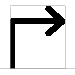
\includegraphics[scale=2.0]{figures/promoter-specification.pdf}

\includegraphics[scale=2.0]{figures/ribosome-entry-site-specification.pdf}
\caption{Examples of glyph specification: this specification for the Promoter glyph (left) and Ribosome Entry Site glyph (right) include the glyph outline, fill (grey center of Ribosome Entry Site), bounding box (dashed box), and recommended alignment with the nucleic acid backbone (dashed horizontal line), all at a preferred relative scale.}
\label{f:specexample}
\end{figure}

\subsection{Reserved Visual Properties}

SBOL Visual aims to allow as much flexibility and freedom as possible in how diagrams are organized, presented, and styled.
%
To this end, a number of aspects of presentation are generally reserved for the communication of other types of information by the creator of a diagram.
%
When using a glyph in a diagram, the following choices in glyph presentation are thus explicitly intended to be alterable:
\begin{enumerate}
\item The lines of a glyph MAY be given any line thickness and style
\item The interior of a glyph MAY be given any fill color.
\item The scale of glyphs are RECOMMENDED to be kept consistent with their specification and throughout a diagram, but can be altered if desired, particularly to convey additional information (e.g., length of a sequence).
\item Minor styling effects MAY be chosen (e.g., shadow, corner styling, other "font-level" customization)
\end{enumerate}
\ref{f:stylevariation} shows some examples of acceptable style variation.

In certain special cases, the style of a glyph may be more constrained, but such cases are expected to be rare and strongly motivated.

\begin{figure}[h!]
\centering

\includegraphics[scale=1.0]{figures/style-variation.pdf}
\caption{Examples of acceptable style variation for a Promoter glyph.}
\label{f:stylevariation}
\end{figure}


\subsection{Extending the Set of Glyphs}\label{sec:extension}
The collection of SBOL Visual glyphs is not expected to provide
complete coverage of all of the types of component that people will
wish to include in genetic diagrams, particularly given the ongoing
evolution of synthetic biology as an engineering discipline.
%
As the need for new diagram elements or new practices of usage emerge,
new glyphs or glyph definitions are expected to be added to SBOL
Visual.
%
In particular, the following three classes of changes are expected to occur regularly,
and the SBOL development community will maintain clear processes for
proposal and adoption of changes of this type:
\begin{itemize}
\item New glyphs, either representing a type of component that
  previously lacked a glyph or enabling a distinction between types of
  component previously represented by the same glyph.
\item Additional glyph variants, accompanied by compelling use cases
  that cannot be adequately addressed by the existing glyph variants.
\item Additional definitions for a glyph, capturing an alternate
  meaning that is useful to humans but existing within a disjoint
  branch of the Sequence Ontology.
\end{itemize}

In order to support the coherent extension of SBOL Visual, 
whenever a diagram creator uses a glyph not found in \ref{apdx:symbols}, 
the creator SHOULD submit it to be considered for inclusion in an updated version of the standard following the processes for adding new glyphs found on the community website at \url{http://sbolstandard.org}



